\chapter{Introduction} \label{chap:intro}

\section*{}

This first chapter aims to provide the reader with an overview of this
dissertation. It starts by introducing the context this work is inserted in,
identifying the problem which we aim to solve, how we plan on solving it, and
the expected outcome. Lastly, it gives a bird's eye view of this report's
structure.

\section{Context} \label{sec:context}

There is, among several domains with interesting and relevant problems to solve
(computer vision \cite{Kulkarni2015}, cryptography, biology, fraud detection,
recommender systems \cite{intml}, ...), the recurring necessity to be able to
make decisions in the face of uncertainty using machine learning (ML) methods.

Successful ML applications include Google's personalized advertising and
context-driven information retrieval, Facebook's studies of how information
spreads across a network or UC Berkeley's AMPLab contributions towards Amazon
Web Services and SAP's products \cite{Broder:2015:BDN:2684822.2697027}.

Typically, there are two alternatives for solving this class of problems: either use an
existing machine learning model (such as KNN, neural networks or similar) \cite{mlnot} and
try to fit your data into the model, or build a probabilistic model for your
own particular problem so you can better leverage domain knowledge \cite{SciPy}.

In the second alternative one common way to approach it is by using bayesian reasoning,
where you model unknown causes with random variables, feed the model the data you
have gathered and then perform inference to query for the
desired, and previously unknown, variables \cite{thbay}. The problem in choosing
this method is this last step, since it is non-trivial
to write an inference method \cite{Duvenaud}.

The solution to this has been building generic inference engines for graphical
models, so that modeling and inference can be treated as separate concerns and
people can focus on the modeling \cite{Jordan1996}. However, not all models can be represented as
graphical models, and that’s why we now have Probabilistic Programming Languages
(PPLs). Probabilistic Programs let you write your model as a program and have
off-the-shelf inference \cite{Prekopa2003}.

\section{Problem} \label{sec:proj}

In spite of these examples of applications in the industry, ML has been
identified by Gartner, in its Hype Cycle annual review,
to be in the "Peak of Inflated Expectations" stage, still far
from the "Plateau of Producitvity" \cite{gartner}.

It has also been said that ML's applications are rarely seen
outside the academia, with Wagstaff claiming that there is a "frequent lack of
connection between machine learning research and the larger world of scientific
inquiry and humanity" \cite{Wagstaff2012}.

Arguably the scenario is even worse for PPLs, having even less adoption
among tech companies than other ML methods, such as neural networks or other
supervised learning models. One factor which may be contributing to this lack of
usage, despite PP's power and flexibility, is the difficulty for data scientists
to adapt to the textual interface these languages provide, which lack the graphical
intuition provided by other tools they are accustomed to. In a poll made to find
out the most popular data-mining tools among data scientists
(see Figure \ref{fig:poll}), half of the top 10 tools are
graphically-interactable.

\begin{figure}[t]
  \begin{center}
    \leavevmode
    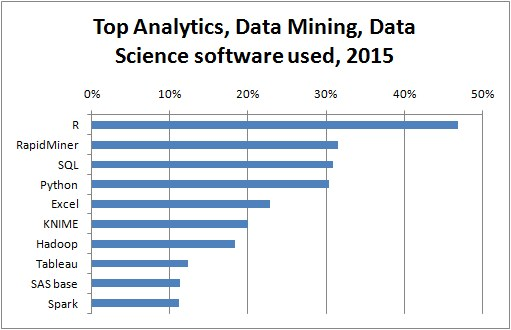
\includegraphics[width=0.86\textwidth]{poll}
    \caption{Top 10 Analytics Tools \cite{kdn}}
    \label{fig:poll}
  \end{center}
\end{figure}

\section{Motivation and Goals} \label{sec:goals}

The Defense Advanced Research Projects Agency (DARPA), one of the backers behind
PPLs' research, has recognized some of the problems
identified by Wagstaff and started a program called Probabilistic Programming
for Advancing Machine Learning (PPAML) to address the shortcomings of
current ML methods \cite{darpa}. It identifies five strategic goals:

\begin{itemize}
  \item Shorten machine learning model code to make models faster to write and
  easier to understand
  \item Reduce development time and cost to encourage experimentation
  \item Facilitate the construction of more sophisticated models that
  incorporate rich domain knowledge and separate queries from underlying code
  \item Reduce the level of expertise necessary to build machine learning
  applications
  \item Support the construction of integrated models across a wide variety of
  domains and tool types
\end{itemize}

The purpose of this work is to try addressing the first four. In order to do so we
aim to overcome the difficulties in learning a new language, either for
inexperienced developers or seasoned ones, such as learning yet another syntax
or getting accustomed to the language's idioms. It is known that typical
languages are difficult to learn and use \cite{Lewis1987} and that there are
advantages in providing a language with a visual interface \cite{dfbeg}. Also,
studies have shown that programmers and data scientists alike resort to mental
imagery when solving problems \cite{Dastani2002}\cite{Petre1999}, so by
providing such an interface we can approximate how people think and how they
use the language to solve the problem at hand.

So, the goal of this dissertation will be to develop a Visual Programming
Language (VPL) with probabilistic programming capabilities. The targeted
audience are programmers and data scientists with background knowledge in
statistics who aren't still comfortable
with full blown PPLs, but wish to educate themselves in the topic so they can
eventually leverage the power of this novel machine learning approach.

The way to do so would be developing a graphical node-based editor, similar to
RapidMiner or Blender Composite Nodes, but that runs in the browser. The given
editor would have the capability to compile its graph to the textual
representation in the target PPL so that the user can run what he has designed,
either as a standalone script or even by integrating it with his existing
projects.

The hypothesis under consideration is this graphical representation
is more intuitive and easy to learn that a full-blown PPL.
We intend to validate such hypothesis by ensuring that classical problems solved
in the literature by PPLs are also supported by our graphical representation,
and then measure how quickly a group of people trained in statistics would
produce a viable model in both alternatives.
